\usetikzlibrary{decorations.pathreplacing}
% Define a macro to collapse the grid drawing block
\newcommand{\drawGrid}{
    % Define the overlap length
    \def\overlap{0.3}
    
    % Draw full opacity dashed grid inside the 2x2 box
    \draw[black, dashed, opacity=1] (0,0) grid (2,2);
    
    % Draw reduced opacity dashed lines extending beyond the 2x2 box with adaptable length
    % Corner extensions
    \draw[black, dashed, opacity=0.3] (2,2) -- (2+\overlap,2);   % Right horizontal extension (top)
    \draw[black, dashed, opacity=0.3] (2,2) -- (2,2+\overlap);   % Top vertical extension (right)
    \draw[black, dashed, opacity=0.3] (0,2) -- (0-\overlap,2);   % Left horizontal extension (top)
    \draw[black, dashed, opacity=0.3] (0,2) -- (0,2+\overlap);   % Top vertical extension (left)
    \draw[black, dashed, opacity=0.3] (2,0) -- (2+\overlap,0);   % Right horizontal extension (bottom)
    \draw[black, dashed, opacity=0.3] (2,0) -- (2,0-\overlap);   % Bottom vertical extension (right)
    \draw[black, dashed, opacity=0.3] (0,0) -- (0-\overlap,0);   % Left horizontal extension (bottom)
    \draw[black, dashed, opacity=0.3] (0,0) -- (0,0-\overlap);   % Bottom vertical extension (left)
    
    % Middle line extensions
    \draw[black, dashed, opacity=0.3] (1,2) -- (1,2+\overlap);   % Middle top vertical extension
    \draw[black, dashed, opacity=0.3] (1,0) -- (1,0-\overlap);   % Middle bottom vertical extension
    \draw[black, dashed, opacity=0.3] (2,1) -- (2+\overlap,1);   % Middle right horizontal extension
    \draw[black, dashed, opacity=0.3] (0,1) -- (0-\overlap,1);   % Middle left horizontal extension
}

\section{Electrostatic Particle in Cell Method}
\label{sec: ES PIC}
As discussed in the previous section, the behavior of plasma in electrostatic fields is governed by Poisson’s equation (see Eq. \ref{Eq: Poissions}). This differential equation rarely has an analytical solution except in simple, idealized cases, requiring numerical methods for accurate simulation in complex practical applications. A common numerical method in this context is the Electrostatic Particle-In-Cell (\acs{ES PIC}) technique, which provides a valuable framework for plasma simulations and can even be extended to electromagnetic codes that solve Maxwell’s equations in their entirety \cite{brieda_plasma_2019}.

Unlike physical plasma phenomena, simulations proceed discontinuously by dividing the physical domain into a fine enough spatial grid. The individual elements of this computational grid are referred to as cells, which collectively form the simulation mesh. The points where the corners of these cells meet are known as nodes and are shared among neighboring cells. Generally, cells can have arbitrary shapes, provided they do not intersect with one another \cite{brieda_plasma_2019}. For the extent of this research, we used a quadratic cell layout in cartesian coordinates, which is advantageous due to its simplicity of implementation but lack the ability to resolve complex geometries. However, curved objects or smooth geometries can be implemented by using the sugarcube method, which allows for an approximation of complex shapes within a cartesian mesh (discussed in Section \ref{Chap: experimenantal part}).

Furthermore, the side length of a cell $\Delta x$ cannot be chosen excessively large but must instead be determined based on the specific objective and external conditions of the system. Generally, all plasmas can be characterized by a fundamental length, known as the Debye length $\lambda_\mathrm{d}$, which is determined by the temperature $T$ and number density $n$ of the charged particles \cite{gurnett_introduction_2017}. Considering a homogeneous plasma, where the ion temperature $T_\mathrm{i}$ is typically much lower than the electron temperature $T_\mathrm{e}$, it is customary to neglect the ion contribution \cite{brieda_plasma_2019}. This leads to the following expression for the Debye length: 
\begin{align}
\lambda_D = \sqrt{\frac{\epsilon_0 k_B T_e}{n_e q_e^2}}\quad\quad k_B &\text{: Boltzmann constant}\\
\intertext{To resolve the local charge density accurately and compute the electric field $\boldvec{E}$, the simulation grid must be sufficiently fine \cite{birdsall_plasma_2005}. Therefore, the cell volume in a \acs{PIC} simulation for plasma flow must be smaller than the volume of the Debye sphere, ensuring accurate resolution \cite{brieda_plasma_2019}:}
(\Delta x \Delta y \Delta z) &< \frac{4}{3} \pi \lambda_D^3
\end{align}

The simulation mesh intrinsically defines discrete points where key properties, such as the density $\rho$, the electric potential $\phi$, or the electric field $\boldvec{E}$, can be determined. While some methods define these points at the cell center, the commonly used node-based approach was employed in this work \cite{brieda_plasma_2019}. A particle within a cell interacts only with its surrounding nodes and is governed by the interpolated mesh data at its specific position within the cell. This approach accordingly enables the interpolation of particle-based data back onto the computational grid. Furthermore, the unique set of boundary conditions for the system is also established through the simulation mesh. Two of the most commonly applied boundary conditions in the context of \acs{PIC} simulations are the Dirichlet and Neumann boundary conditions. The Dirichlet boundary condition specifies the value of the function itself, such as the electric potential \cite{press_numerical_2007}. On the other hand, a Neumann boundary condition defines the values of the normal gradients on the boundary, implying that there is a predefined behavior in the direction perpendicular to the boundary \cite{press_numerical_2007}. Other types of boundary conditions include Robin, Cauchy, and mixed versions of both, though they are used less frequently in most applications \cite{brieda_plasma_2019}.

\begin{figure}[H]
    \centering
    \begin{tikzpicture}[scale=1.8]
    
    % Left Grid
    \drawGrid

    % Right Grid (shifted to the right by 4 units)
    \begin{scope}[xshift=4cm]
        \drawGrid
        \def\tolerance{0}

% Define the particle position
\def\particleX{1.6}
\def\particleY{0.8}

% Draw arrows from surrounding blue nodes to the green particle using 'latex' arrow tips
\draw[ thick, line width=1] (1+\tolerance,0+\tolerance) -- (\particleX-\tolerance,\particleY-\tolerance);  % Bottom-left node to particle
\draw[ thick, line width=1.1] (2-\tolerance,0+\tolerance) -- (\particleX+\tolerance,\particleY-\tolerance);  % Bottom-right node to particle
\draw[ thick, line width=1.5] (1+\tolerance,1-\tolerance) -- (\particleX-\tolerance,\particleY+\tolerance);  % Top-left node to particle
\draw[thick, line width=1.2] (2-\tolerance,1-\tolerance) -- (\particleX+\tolerance,\particleY+\tolerance);  
% Draw the particle
\fill[thmgreen,draw=black] (1.6,0.8) circle (3pt);  % Red particle with radius 3pt
\node[above] at (1, 2.3) {\textcolor{black}{cells}}; % Label "nodes" above the points

% Draw arrows from the "nodes" label to the blue points with a bit of spacing
\draw[-latex, thick] (.9, 2.3) -- (0.4, 1.5);  % Arrow to the leftmost blue point with some space
\draw[-latex, thick] (1.1, 2.3) -- (1.6, 1.5);  % Arrow to the middle blue point with some space

    \end{scope}

    % Draw the arrow and the text between the grids
    \draw[-latex,thick] (2.3,1) -- (3.7,1); % Arrow between the grid
    \node at (3,1.2) {next iteration};  % Text above the arrow

\draw[-latex,thick,red, line width=1.7] (0.45,0.3) -- (1.6,0.8) node[below] {$F_i$};

    % Define a tolerance for arrow starting and ending positions
\def\tolerance{0.00}

% Define the particle position
\def\particleX{0.4}
\def\particleY{0.3}

% Draw arrows from surrounding blue nodes to the green particle using 'latex' arrow tips
\draw[ thick, line width=0.8] (0+\tolerance,0+\tolerance) -- (\particleX-\tolerance,\particleY-\tolerance);  % Bottom-left node to particle
\draw[ thick, line width=1.1] (1-\tolerance,0+\tolerance) -- (\particleX+\tolerance,\particleY-\tolerance);  % Bottom-right node to particle
\draw[ thick, line width=1.1] (0+\tolerance,1-\tolerance) -- (\particleX-\tolerance,\particleY+\tolerance);  % Top-left node to particle
\draw[thick, line width=1.5] (1-\tolerance,1-\tolerance) -- (\particleX+\tolerance,\particleY+\tolerance);  
% Draw the particle
\fill[thmgreen,draw=black] (0.4,0.3) circle (3pt);  % Green particle with black outline and radius 3pt

% Add the label above the particle with black font
\node[left] at (0.32, 0.3) {\textcolor{black}{$\boldvec{E}_i$}};

\node[above] at (1, 2.3) {\textcolor{black}{nodes}}; % Label "nodes" above the points

% Draw arrows from the "nodes" label to the blue points with a bit of spacing
\draw[-latex, thick] (.9, 2.3) -- (0.1, 2.04);  % Arrow to the leftmost blue point with some space
\draw[-latex, thick] (1.0, 2.3) -- (1.96, 1.06);  % Arrow to the rightmost blue point with some space
\draw[-latex, thick] (1.1, 2.3) -- (1.93, 2.03);  % Arrow to the middle blue point with some space
\draw[thick, decorate, decoration={brace, amplitude=7pt}] (-0.07,1) -- (-0.07,2) node[midway, left=8pt] {$\Delta x$};

    % Blue points for the left grid
    \foreach \x in {0,1,2}
        \foreach \y in {0,1,2}
            \fill[jlublau] (\x,\y) circle (1.7pt);  % Blue points with radius 2pt
    
    % Blue points for the right grid
    \foreach \x in {0,1,2}
        \foreach \y in {0,1,2}
            \fill[jlublau] (\x+4,\y) circle (1.7pt);  % Shift the blue points to the right for the second grid



    \end{tikzpicture}
    \caption{Visualization of the Electrostatic (\acs{PIC}) method for a single particle inside a 2x2 cell grid. The electric Field at each node contributes to the total electric field $\boldvec{E}_\mathrm{i}$ at the position $\boldvec{r}_\mathrm{i}$ which is then used to compute the resulting force $\boldvec{F}_\mathrm{i}$ acting on the particle. The particle's position and velocity are updated iteratively at each time step.}
    \label{fig:grid}
\end{figure}

Similar to the requirements on the cell size $\Delta x$, the simulation scheme generally divides the temporal dimension into discrete states, each separated by a small time step $\Delta t$. Firstly, the time step must be sufficiently small to account for the fastest relevant frequency, which corresponds in the case of fully kinetic studies to the plasma frequency $\omega_\mathrm{pe}$:

\begin{align}
\Delta t &\ll \frac{1}{\omega_\mathrm{pe}}\\
\intertext{Secondly, the time step must ensure that particles do not travel more than one cell length per iteration step, as this would lead to discontinuity problems in the electric field experienced by the particle. Due to their smaller mass, electrons move significantly faster than ions in fully kinetic simulations \cite{brieda_plasma_2019}. Thus, the time step must satisfy the following condition:}
\Delta t &< \frac{\Delta x}{v_{\mathrm{max}}}
\end{align}
\newline
\begin{figure}[H]
    \centering
    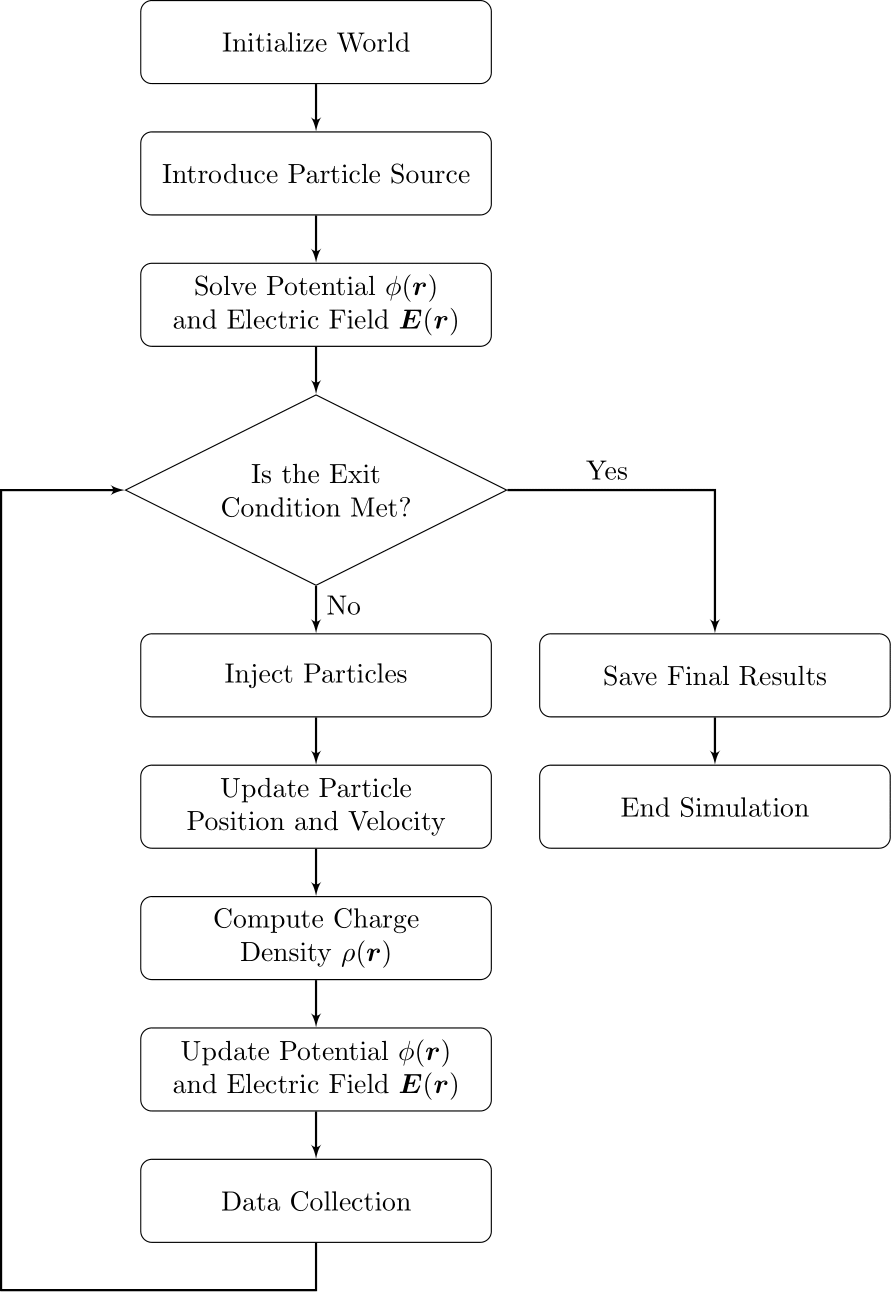
\includegraphics[width=0.65\linewidth]{figures/chapter 2/Flowchart_Studienprojekt with rho.png}
    \caption{Representation of the iterative Particle-in-Cell (\acs{PIC}) simulation process.}
    \label{fig: Flowchart}
\end{figure}

The Particle-in-Cell (\acs{PIC}) scheme employed in this research begins by initializing the discrete simulation domain and introducing the relevant particles. The initial charge and current densities are used to calculate the fields, which in turn enable the movement of particles (outlined in Section \ref{Sec: Particle Motion}). The fields are recalculated at each iteration based on the particles' updated positions and velocities. For simplicity, inter-particle collisions are not considered in this model. However, methods such as Monte Carlo Collisions (\acs{MCC}) and Direct Simulation Monte Carlo (\acs{DSMC}) can be implemented to account for these effects \cite{brieda_plasma_2019,birdsall_particle--cell_1991}. Furthermore, particles that exit the computational domain are either removed or reflected back, depending on the specific requirements of the simulation.

Practical plasma systems typically involve such an immense number of particles that simulating each particle individually becomes computationally impractical \cite{brieda_plasma_2019}. To address this, macroparticles are employed, each of which represents a large number of real particles. Each simulation particle is assigned a constant macroparticle weight $w_\mathrm{mp}$, which represents the number of real ions, electrons, or atoms it corresponds to. Each macroparticle can be envisioned as a cluster of $w_\mathrm{mp}$ real ions or electrons, all moving together with a shared position $\boldvec{x}_\mathrm{mp}$ and momentum $\boldvec{p}_\mathrm{mp}$ \cite{wu_particle--cell_2018}. Given that macroparticle weighting has no impact on the charge-to-mass ratio, the representative simulation particle moves along the same trajectory as the \textit{real} plasma particle.

\begin{equation}
    w_\mathrm{mp} = \frac{N_\mathrm{real}}{M_\mathrm{sim}}
\end{equation}


%\section{Discretize World Domain}
